\chapter{Hardware Used in Creating the Application}
During early development we looked at different hardware and software, in order to figure out what exactly we wanted to do.
We looked at the Kinect by Microsoft, Myo Armband by Elliptic Labs, Leap Motion by Leap Motion Inc and Alexa Voice Assistant by Amazon.

After looking into Myo and Kinect both had the problem were they had been discontinued. Myo has been entirely discontinued with their  website 'http://www.myo.com' is offline (Although their support site is still online for current users to download drivers). 
Kinect has been discontinued on windows and Microsoft consoles Xbox 360/One. Since the Xbox One S Microsoft have removed the port required by the Kinect and have stopped selling the adapter necessary for the Kinect to operate.

That left us with the Leap Motion and the Alexa family of devices.
We looked into what we thought would be more beneficial to learn and looked at Google trends to see which has a more Market viable skill to learn.

\begin{figure}[h!]
  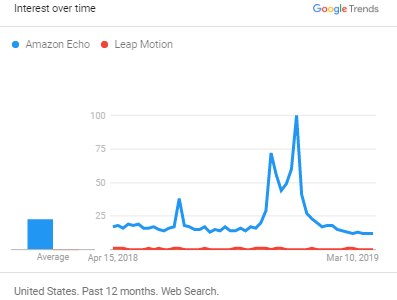
\includegraphics[width=\linewidth]{Stat.PNG}
  \caption{Google Trends}
  \label{fig:googletrends}
\end{figure}

After looking at a graph like this we can clearly see that Alexa is a more searched term over Leap Motion. With this we though that Alexa would be a better choice over Leap Motion.

\section{Echo Input - Echo Plus (Audio only)}
\begin{figure}[h!]
  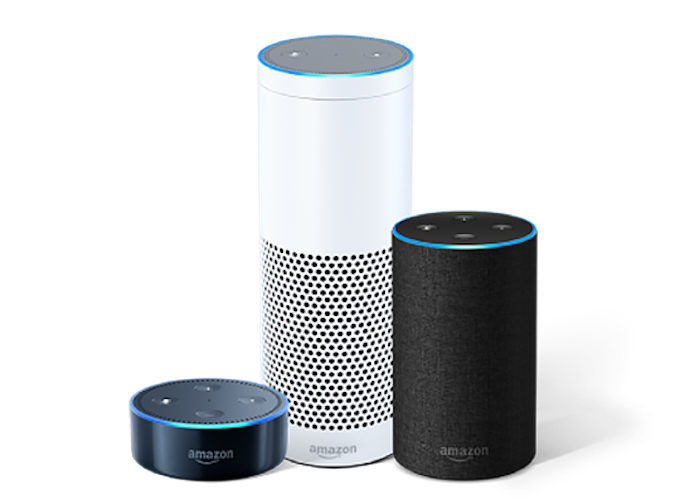
\includegraphics[width=10cm,height=10cm,keepaspectratio]{audio.png}
  \caption{Echo Audio Only}
  \label{fig:echoaudioonly}
\end{figure}

We initially started development with the intent to only develop for Echo devices with audio only, although the skill would still work on the visual models but with audio only. The entire project was built with these models in mind and only later did we add support for visual models.

\section{Echo Show \& Echo Spot (Visual)}
\begin{figure}[h!]
  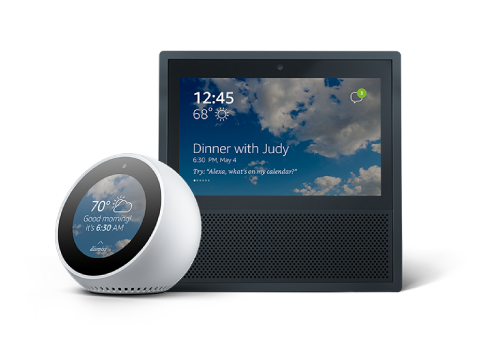
\includegraphics[width=10cm,height=10cm,keepaspectratio]{showSpot.png}
  \caption{Echo Audio Only}
  \label{fig:echoaudioonly}
\end{figure}

A the project went on an we came to terms on how exactly the Alexa voice assistant works and how it handles user interaction, we became more confident in adding more features to it. We figured out how to add a user interface by creating a basic user interface layout that we could call and add the data we needed to the user interface. This system worked very similar to how to tell Alexa to say a certain phrase, but with a few extra variables for title, text, small image and large image. Using these settings we can give more information to the user if they have an Alexa device with a screen such as the game box art.

\begin{figure}[h!]
  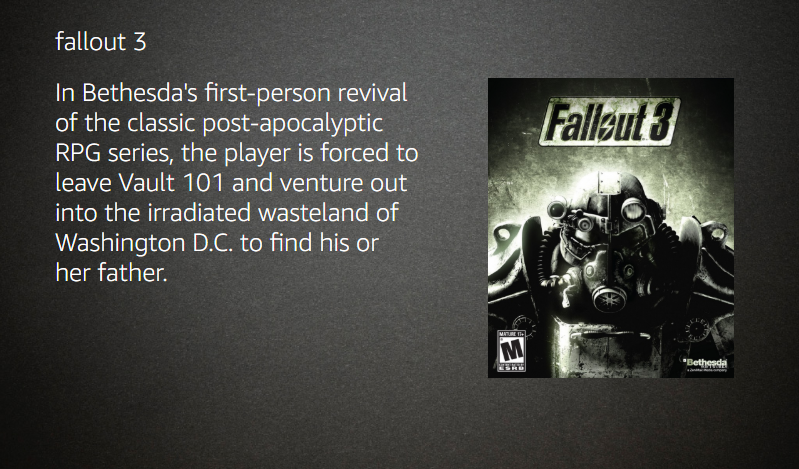
\includegraphics[width=\linewidth]{game.png}
  \caption{Game Intent}
  \label{fig:gameintent}
\end{figure}

As you see above an example of how the user interface will look when a user says 'Alexa ask game finder what is fallout 3'. The user interface will display the title of the game, a description and the game box art. We added this part to include all Alexa enabled devices on the market. Even though Alexa would still work without a user interface when we tested the skill on the Echo Show we found it didn't seem right when every other application had a user interface for these devices and ours had just audio.